\section{Model 1}\label{sec:model-1}
Model 1 is inspired by a model purposed by Claisse and Frey \cite{Claisse-Frey} which inspired this thesis. They introduced a distance-dependent function that were linearly dependent on an unsigned distance function to the point set. We thus look at a function
\begin{equation*}
    \hat{f}_1(d(\mathbf{x};\pointsetm)) = d(\mathbf{x};\pointsetm).
    \label{eq:pure-dist-model}
\end{equation*}

As stated above, a distance dependent function which is positive everywhere would yield no optimal curve satisfying $\diff E(\Omega) = 0$ except for the trivial zero solution. Also for the attraction term defined above, we see from \eqref{eq:general-normal-velocity} that even when the curve is inside the point set, the velocity would have direction inwards. A natural choice is then to define the distance to be negative inside the point set, thus yielding a curve moving outwards when inside the point set.

This brings us to an interesting question. How do we determine what is on the inside or outside of a set of points? When we discussed the signed distance function, the distance was related a closed curve which has a defined inside. When there is only points, we must be able to draw the boarder between the inside and outside in some way, which means that we must construct a closed curve from the set of points.

We denote the constructed closed curve as $\mathcal{C}_\mathcal{V}$ and thus the signed distance to the curve is $u_d(\mathbf{x}; \mathcal{C}_\mathcal{V})$. Assuming then that we can construct such a curve, we define the distance dependent velocity as 
\begin{equation}
    \tilde{f}_1(d(\mathbf{x};\pointsetm)) = u_d(\mathbf{x}; \mathcal{C}_\mathcal{V}).
    \label{eq:signed-dist-model}
\end{equation}

This may seem like a nice solution. Outside the curve $\mathcal{C}_\mathcal{V}$, the curve, \curve, will be pulled inwards by \eqref{eq:signed-dist-model}, and oppositely it will be pulled outwards if inside $\mathcal{C}_\mathcal{V}$. With no curvature dependent term, we would expect a final curve exactly equal $\mathcal{C}_\mathcal{V}$, and with the curvature term, one could expect a smoother but similar solution. 

The problem is, that we are looking for a curve that can approximate any set of points without assumptions on the structure of the sample points. Without information about the connection between the data points, we can not construct for example a polygon from the data points, which would have been a natural choice. 

Hence, because \eqref{eq:signed-dist-model} do not correspond well with the assumptions for the thesis, we approach the problem differently. With no information about the distribution of points, we go back to the unsigned distance function applied to our point set \distanceV. At all points $\mathbf{x}\in\realspacem^2$, \distanceV\ provides the distance to the closest sampled point in \pointset. Now the speed is decided by the distance to the closest point, and we want to construct a sign function $\sigma(\mathbf{x})$ that determines the direction of the speed in order to pull the curve towards its closest point without making any assumptions on the composition of the data points.

To construct such a sign function, recognize that the only movement we are interested in is the movement of the zero isocontour. Thus the sign function needs only to have a reasonable sign for the values at the zero level curve. We can thus turn the problem around. Rather than figuring out if the curve is inside the point set, we detect whether or not the points in the point set is outside the zero level curve. The curve, \curve, is closed and thus has a meaningful inside and outside. In addition, by construction the sign of \uxt\ is negative inside \curve\ and oppositely positive outside as seen in \eqref{eq:interior}-\eqref{eq:exterior}. 

Using this, we construct the sign function $\sigma(\mathbf{x})$ as follows. For a fixed $t=t^*$, then for every part of the curve $\Gamma(t^*)_r$, denote $\mathbf{v}_r$ as the closest sample point. Then $\sigma(\Gamma(t^*)_r) = \texttt{sgn}(u(\mathbf{v}_r, t^*))$. Because the position of the curve relative to the sample points changes over time, we construct a time dependent sign function that we extend to the entire domain \domain\ as follows:
\begin{equation}
    \sigma(\mathbf{x}, t) = \texttt{sgn}((u(\mathbf{v}_r, t))), \quad \mathbf{v}_r = \texttt{argmin}(\|\mathbf{x}- \mathbf{v}\|_2 \, \forall \mathbf{v} \in \pointsetm). 
    \label{eq:sigma-def}
\end{equation}\todo{figur av sigma som vil se ut som kakestykker}

Using the above, we end up with a model that will draw the curve towards the closest sample points. The distance dependent velocity for model 1 is then defined as
\begin{equation}
    f_1(d(\mathbf{x};\pointsetm)) = \sigma(\mathbf{x}, t) d(\mathbf{x};\pointsetm),
    \label{eq:model1-dist-velocity}
\end{equation}
yielding the full model, by inserting \eqref{eq:model1-dist-velocity} into \eqref{eq:general-model-pde}: \\
\begin{tcolorbox}[title=Model 1]
\begin{equation}
    u_t = |\nabla u|(\alpha\sigma(\mathbf{x}, t) d(\mathbf{x}; \pointsetm) + (1-\alpha) \kappa(x)), \quad \alpha \in \realspacem
    \label{eq:model1-pde}
\end{equation} 
\end{tcolorbox}

\textbf{Remark:} The way $\sigma(\mathbf{x}, t)$ is defined in \eqref{eq:sigma-def} will violate the assumptions in Proposition \ref{prop:shape-derivative} and thus we can not find $\diff E_1$ for this choice of $f(d(\mathbf{x};\pointsetm))$ using the proposition. The sign function makes $f$ discontinuous which makes the velocity discontinuous. This was not mentioned by Claisse and Frey \cite{Claisse-Frey} in their Lemma 2.1, which as we read it must have the same issue. 

As the we will see later, this does not damage the numerical results. The discretized velocity will anyways be discontinuous and thus, as long as the grid size is bounded away from zero, the discontinuity is not detectable. When the grid size is is bigger than some bounding $\epsilon>0$, one can construct a smoothing function, $\tilde{\sigma}$, connecting $\sigma=1$ and $\sigma=-1$ with a bounded derivative which is thus in $L^1$. The resulting velocity will then be continuous and for the discretization, $\sigma=\tilde{\sigma}$. This discrepancy between the theory and the model was found rather late in the process and could be something to look into for further work.


%%%%%%%%%%%%%%%%%%%%%%%%%%%%%%%%%%%%%%
\begin{comment}
We see from \eqref{eq:model1-pde} that the curve will have an inward velocity dependent on the distance to the point set and the curvature. In order to draw the curve towards the point set, the sign function $\sigma$ must be positive when the curve is outside the point set. In that case the distance term is contributing to the inward velocity. 

In the opposite case, when the curve is on the inside, the distance term should contribute to an outward-pointing velocity. This meaning $\sigma(\mathbf{x}, t)$ must be negative. Thus the sign function is clearly defined when the whole curve is outside or inside the point set. When parts of the curve is inside, and other parts are outside of the point set, or when it is hard to define what is outside and inside, this is more complex. 

Claisse and Frey makes no mention of what is done when this is the case, other than that the sign function must be defined locally. Hence, it must be both space and time-dependent. We have made a choice regarding the sign function and decided that the value of the sign function should be dependent on whether or not the closest point in the point set is inside or outside the curve. 

This in practice, means that the curve will always be attracted to the closest point in the point set, which seems like a natural choice because the distance function also is the distance to the same point. 
\end{comment}
\subsection{Radially Symmetric Analysis}
We now reduce the situation down to a radially symmetric setting to perform some simplified analysis of the energy function. The setup can be viewed in \figref{fig:stationary-example}, where we have a circular curve $\Gamma(t)$ with radius \radgamma\ and center in the origin. The point set, \pointset, is also distributed in a circle around the same center and with radius $r_v$. Further more, we assume that the density of the point set is so high that we can approximate the set of point as a continuous curve denoted $\Gamma_{\mathcal{V}}$.

\begin{figure}
    \centering
    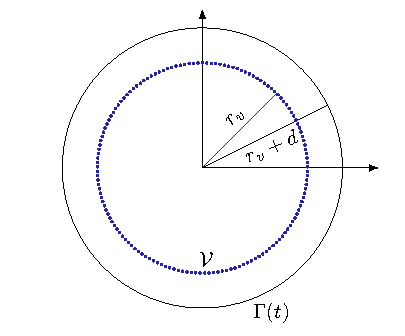
\includegraphics[width=.4\linewidth]{figures/tikz-figures/stationary-example.tex}
    \caption[One dimensional analytical example]{A radially symmetric set up with the point set, $\Gamma_{\pointsetm}$, and curve, $\Gamma (t)$ centered around the origin with radii independent of the angle with respect to the $x$-axis.}
    \label{fig:stationary-example}
\end{figure}
Because of the symmetry and the high density assumption, there will be no spatial discontinuities because the entire curve will either be inside or outside the point set. The resulting \sigmaxt\ will thus be constant in space. Now the energy function $E$ is only a function of \radgamma, and is written
\begin{equation*}
    E(r_{\Gamma}) = \underbrace{\alpha \int_0^{r_{\Gamma}} \texttt{sgn}\{r-r_v\} (r-r_v) 2\pi r \diff r}_\text{$E_1$} + \underbrace{(1-\alpha)\cdot 2\pi r_{\Gamma} \vphantom{ \int_0^{r_{\Gamma}}}}_\text{$E_2$}
\end{equation*}
\begin{equation}
    E(r_{\Gamma}) = \begin{cases}
        2\pi \alpha \bigg( \frac{r_{\Gamma}^3}{3}- \frac{r_{\Gamma}^2 r_v}{2} \bigg) + 2\pi (1-\alpha) r_{\Gamma} &\qquad \text{if } r_{\Gamma}\leq r_v\\
        \frac{2\pi \alpha r_v^3}{3} + 2\pi \alpha \bigg( \frac{r_{\Gamma}^3}{3}- \frac{r_{\Gamma}^2 r_v}{2} \bigg) + (1-\alpha) 2\pi r_{\Gamma} &\qquad \text{if } r_{\Gamma}>r_v
        \end{cases}
    \label{eq:J-rad}
\end{equation}
The total energy function is displayed in \figref{fig:model-jtot} with its separate terms displayed in \figref{fig:model1-j1} for specific parameters $\alpha=0.85$ and $r_v=1$. Here, we see that the energy function does obtain a minimum besides the trivial solution and moreover it is the global minimum. Note also that it is not obtained where $\radgammam=r_v$, but inside the point set, where $\radgammam<r_v$.

\begin{figure}
    \begin{subfigure}[b]{0.48\linewidth}
        \centering
        \includegraphics[width=\linewidth]{figures/Model-1/Jis.tex}
        \caption{The separate energy terms}
        \label{fig:model1-j1}
    \end{subfigure}
    \begin{subfigure}[b]{0.48\linewidth}
        \centering
        \includegraphics[width=\linewidth]{figures/Model-1/J.tex}
        \caption{Total energy function}
        \label{fig:model-jtot}
    \end{subfigure}
    \caption[Minimization problem]{The potential energy function for model 1 \eqref{eq:J-rad} in the radially symmetric situation with $\alpha=0.85$ and $r_v=1$}
    \label{fig:minimization-model1}
\end{figure}

We stick to this radially symmetric situation, and we will see that in one dimensions, \eqref{eq:general-model-pde} is a hyperbolic conservation law.

\subsection*{Method of characteristics}
A scalar hyperbolic conservation is a PDE that can be written in the form 
\begin{equation}
    u_t + \diff f(u) \nabla u = 0,
    \label{eq:general-hyp-cons}
\end{equation}
where $f=(f_1,\dots, f_m)$ and $x=(x_1, \dots, x_n)$\cite{MR3443431}. This can not be done for \eqref{eq:model1-pde} which defines our model in the two-dimensional case because the curvature term is parabolic. However, in the one-dimensional case the curvature reduces to
\begin{equation*}
    \nabla \cdot \frac{\nabla u}{|\nabla u|} = \bigg( \frac{u_x}{|u_x|} \bigg)_x = (\pm 1)_x = 0.
\end{equation*}
We immediately get that \eqref{eq:model1-pde} turns into
\begin{equation*}
    u_t = \pm u_x \alpha \sigma(x) d(x; \pointsetm),
\end{equation*}
which for a $\diff f(u) = \mp \alpha \sigma d(x; \pointsetm)$ is a hyperbolic conservation law as in \eqref{eq:general-hyp-cons}. Because the curvature term is meaningless in one dimensions, this is less interesting seen as it is a key feature for our model. 

In a radially symmetric situation, the curvature is more interesting. The setup is the same as in the calculations leading up to \eqref{eq:J-rad} an is shown in \figref{fig:stationary-example}. For both \pointset\ and $\Gamma$ being circles with the same center, the distance $d(r; \pointsetm) = |r-r_v|$ and the curvature of a circle is known as
\begin{equation}
    \kappa(r) = \frac{1}{r}
    \label{eq:curvature-circle}
\end{equation}
\begin{comment}
\subsection{1 spatial dimension}
\begin{figure}
    \centering
    \includegraphics{figures/tikz-figures/characteristics-1d-initial.tex}
    \caption[Method of characteristics - initial function]{Caption}
    \label{fig:1d-char}
\end{figure}

We look at our equation \todo{ref} in one dimensions. The situation is as pictured in \figref{fig:1d-char}, with the point set consisting of two points, $\mathcal{V}=\{v_1, v_2\}$. We can then assume without loss of generality that they are placed symmetric around the origin. First of all, we notice that in one dimensions, the notion of curvature is meaningless.
\begin{equation}
    \kappa(u) = \Bigg( \frac{u_x}{|u_x|} \Bigg)_x = (\pm 1)_x = 0
\end{equation}

We then have that our level set equation simply is
\begin{equation}
    u_t =\alpha \sigma (x) d(x)\, u_x
\end{equation}

Because our problem is symmetric, the function, $\sigma (x) = \pm 1$, depending on our initial function has a level set that is inside or outside the point set. 

\end{comment}
The term $|\nabla u|$ can be expressed in terms of $r$ through a simple change of variables:
\begin{align*}
    r &=\sqrt{x^2+y^2} \\
    \implies \frac{dr}{dx} &= \frac{x}{\sqrt{x^2 + y^2}} \\
    \implies \frac{dr}{dy} &= \frac{y}{\sqrt{x^2+ y^2}} \\
    |\nabla u| &= \sqrt{u_x^2 + u_y^2} = \sqrt{\frac{\partial u}{\partial r} \frac{dr}{dx} + \frac{\partial u}{\partial r} \frac{dr}{dy}}
\end{align*}
\begin{equation}
    \implies |\nabla u | = \sqrt{\frac{u_r^2}{x^2+y^2} (x^2 + y^2)} = u_r, \qquad \text{if } u_r\geq 0
    \label{eq:nablau-ur}
\end{equation}

Inserting \eqref{eq:curvature-circle} and \eqref{eq:nablau-ur} into \eqref{eq:model1-pde} we get
\begin{equation}
    u_t = u_r \bigg(\alpha \sigma(t)|r-r_v| + \frac{(1-\alpha)}{r} \bigg).
    \label{eq:zero-levelset-polar-coords}
\end{equation}

We have now a conservation law on the form \eqref{eq:general-hyp-cons} for $r$. Because our PDE now is only dependent on the radius, the total derivative of \eqref{eq:zero-levelset-polar-coords} with respect to time becomes
\begin{equation}
    \frac{du}{dt} = u_t + u_r \,r_t.
    \label{eq:polar-characteristic-eq}
\end{equation}

We want to investigate how the curve moves in time. The curve is always the zero level set, and is thus by definition constant and equal to zero. Moreover, the PDE can be even simplified further at the curve because we have that $\sigma(t)(|r_{\Gamma}-r_v|) = (r_{\Gamma}-r_v)$ at the curve, since the sign function changes at the point when $r_{\Gamma}=r_v$. Thus 
\begin{equation}
    u_t = u_r \bigg(\alpha (r-r_v) + \frac{(1-\alpha)}{r} \bigg) \qquad \text{for } r=\radgammam.
    \label{eq:levelset-polar-coords}
\end{equation}
Because of the constant value for $u$ at all level curves, the left hand side in \eqref{eq:polar-characteristic-eq} equals zero. And thus
\begin{equation}
    u_t=-u_r\, r_t,
    \label{eq:characteristic-streamline}
\end{equation}
and by comparing \eqref{eq:characteristic-streamline} with \eqref{eq:zero-levelset-polar-coords}, we see that
\begin{equation}
    r_t = -\bigg(\alpha \sigma|r(t)-r_v| + \frac{(1-\alpha)}{r(t)}\bigg),
    \label{eq:pde-streamline}
\end{equation}
where $r(t)$ is the radius for a single iso-contour which moves in time. We will call the trajectories of the curves following \eqref{eq:pde-streamline}, the streamlines for the solution. First, we want to analyze how the zero level curve moves given an initial radius, $r_0$. We then compare  \eqref{eq:levelset-polar-coords} and \eqref{eq:zero-levelset-polar-coords} to obtain the PDE for the streamline of a zero iso-contour
\begin{equation}
    r_t = -\bigg(\alpha (r(t)-r_v) + \frac{(1-\alpha)}{r(t)}\bigg) \quad \text{for }r(t) = r_{\Gamma}.
    \label{eq:pde-zero-streamline}
\end{equation}

The equation \eqref{eq:pde-zero-streamline} is a separable equation, and the solution is an implicit function of $r(t)$,
\begin{equation}
    \frac{\ln(\alpha(r(t)^2-r_v\,r(t)-1)+1) - \frac{2\sqrt{\alpha}\,r_v \tan^{-1}\bigg(\frac{\sqrt{\alpha} (r_v-2r(t))}{\sqrt{4-\alpha(r_v^2+4)}}\bigg)}{\sqrt{4-\alpha(r_v^2+4)}}}{2\alpha}=-t+C,
    \label{eq:streamline-solution}
\end{equation}
where the constant $C$ is decided from the initial conditions, $t=0$, $r=r_0$.
\begin{equation}
    C=\frac{\ln(\alpha(r_0^2-r_v r_0-1)+1) - \frac{2\sqrt{\alpha}\,r_v \tan^{-1}\bigg(\frac{\sqrt{\alpha} (r_v-2r_0)}{\sqrt{4-\alpha(r_v^2+4)}}\bigg)}{\sqrt{4-\alpha(r_v^2+4)}}}{2\alpha}.
    \label{eq:streamline-solution-constant}
\end{equation}

\begin{figure}
    \begin{subfigure}[b]{0.48\linewidth}
    \centering
        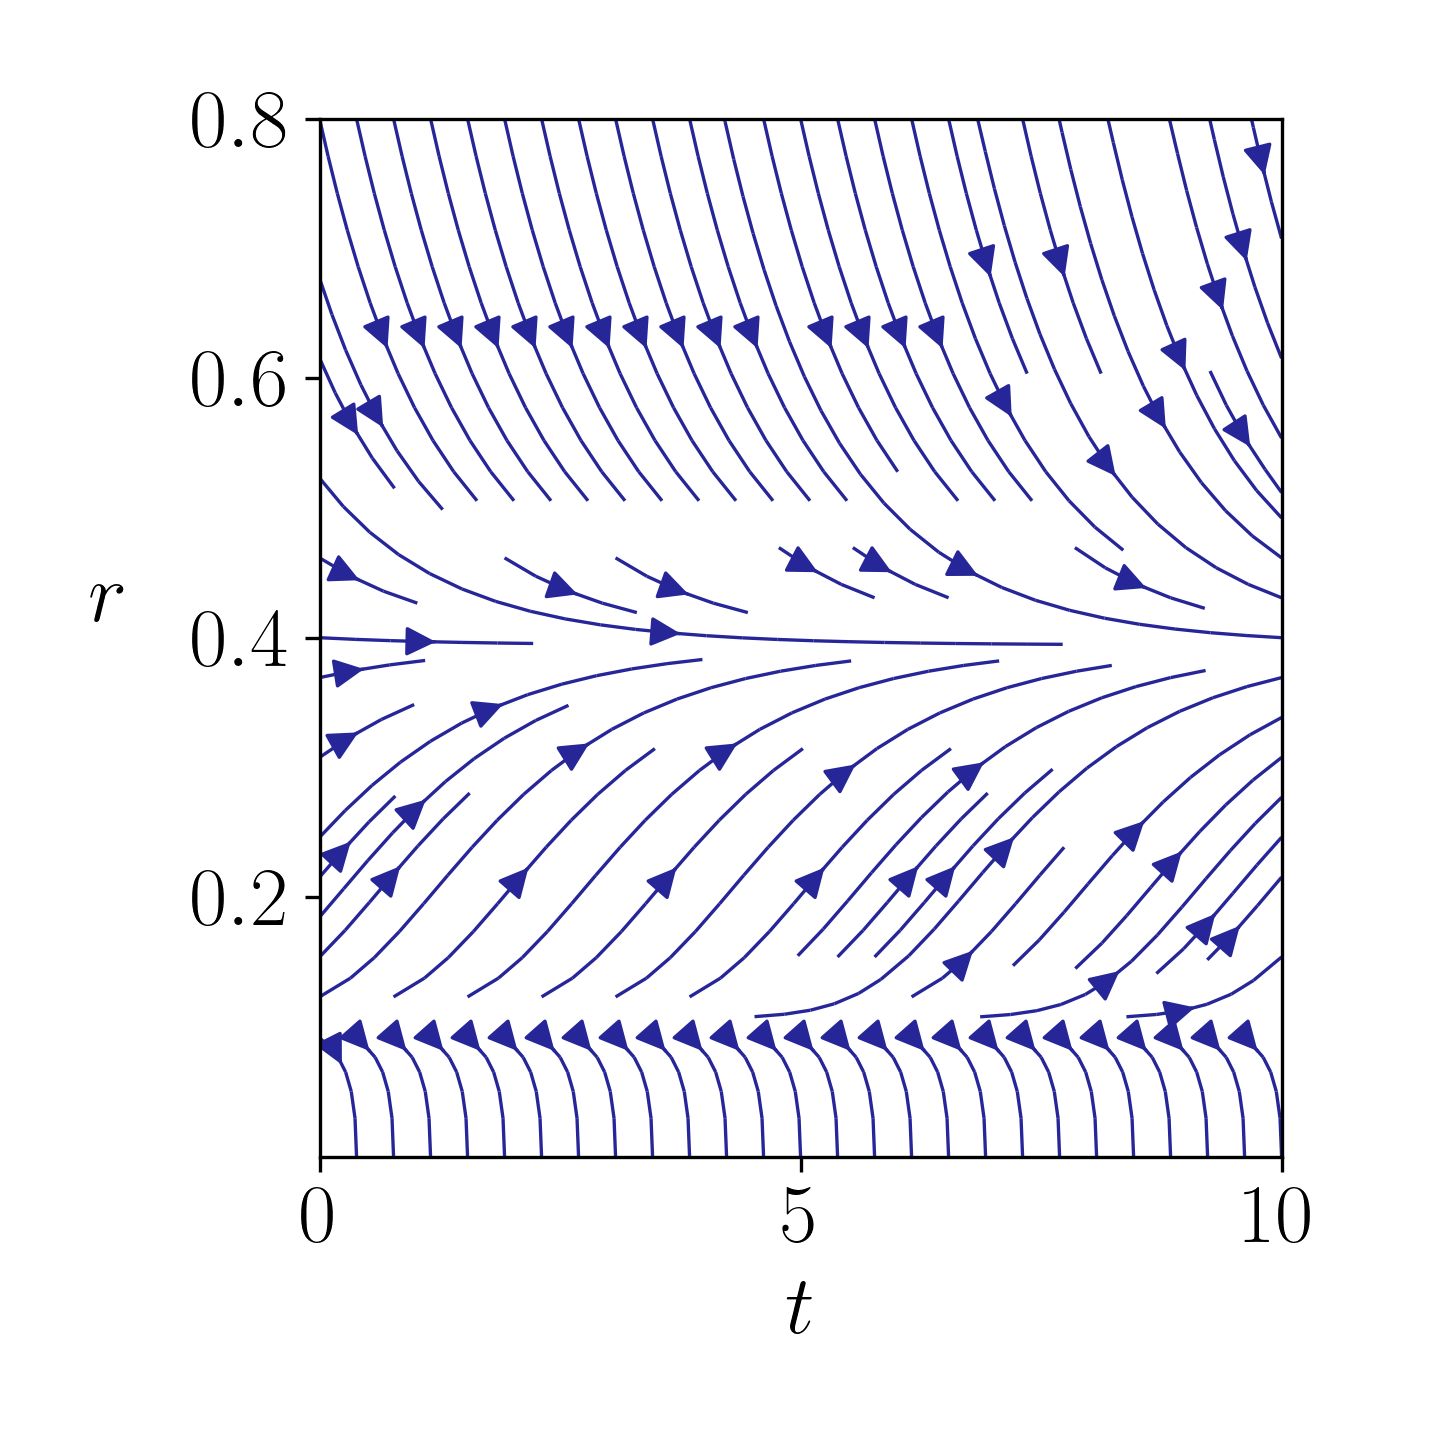
\includegraphics[width=\linewidth]{figures/streamlines/mod1-a96.png}
        \caption{$\alpha=0.96$} 
        \label{fig:radius-characteristics-96} 
    \end{subfigure}
    \begin{subfigure}[b]{0.48\linewidth}
    \centering
        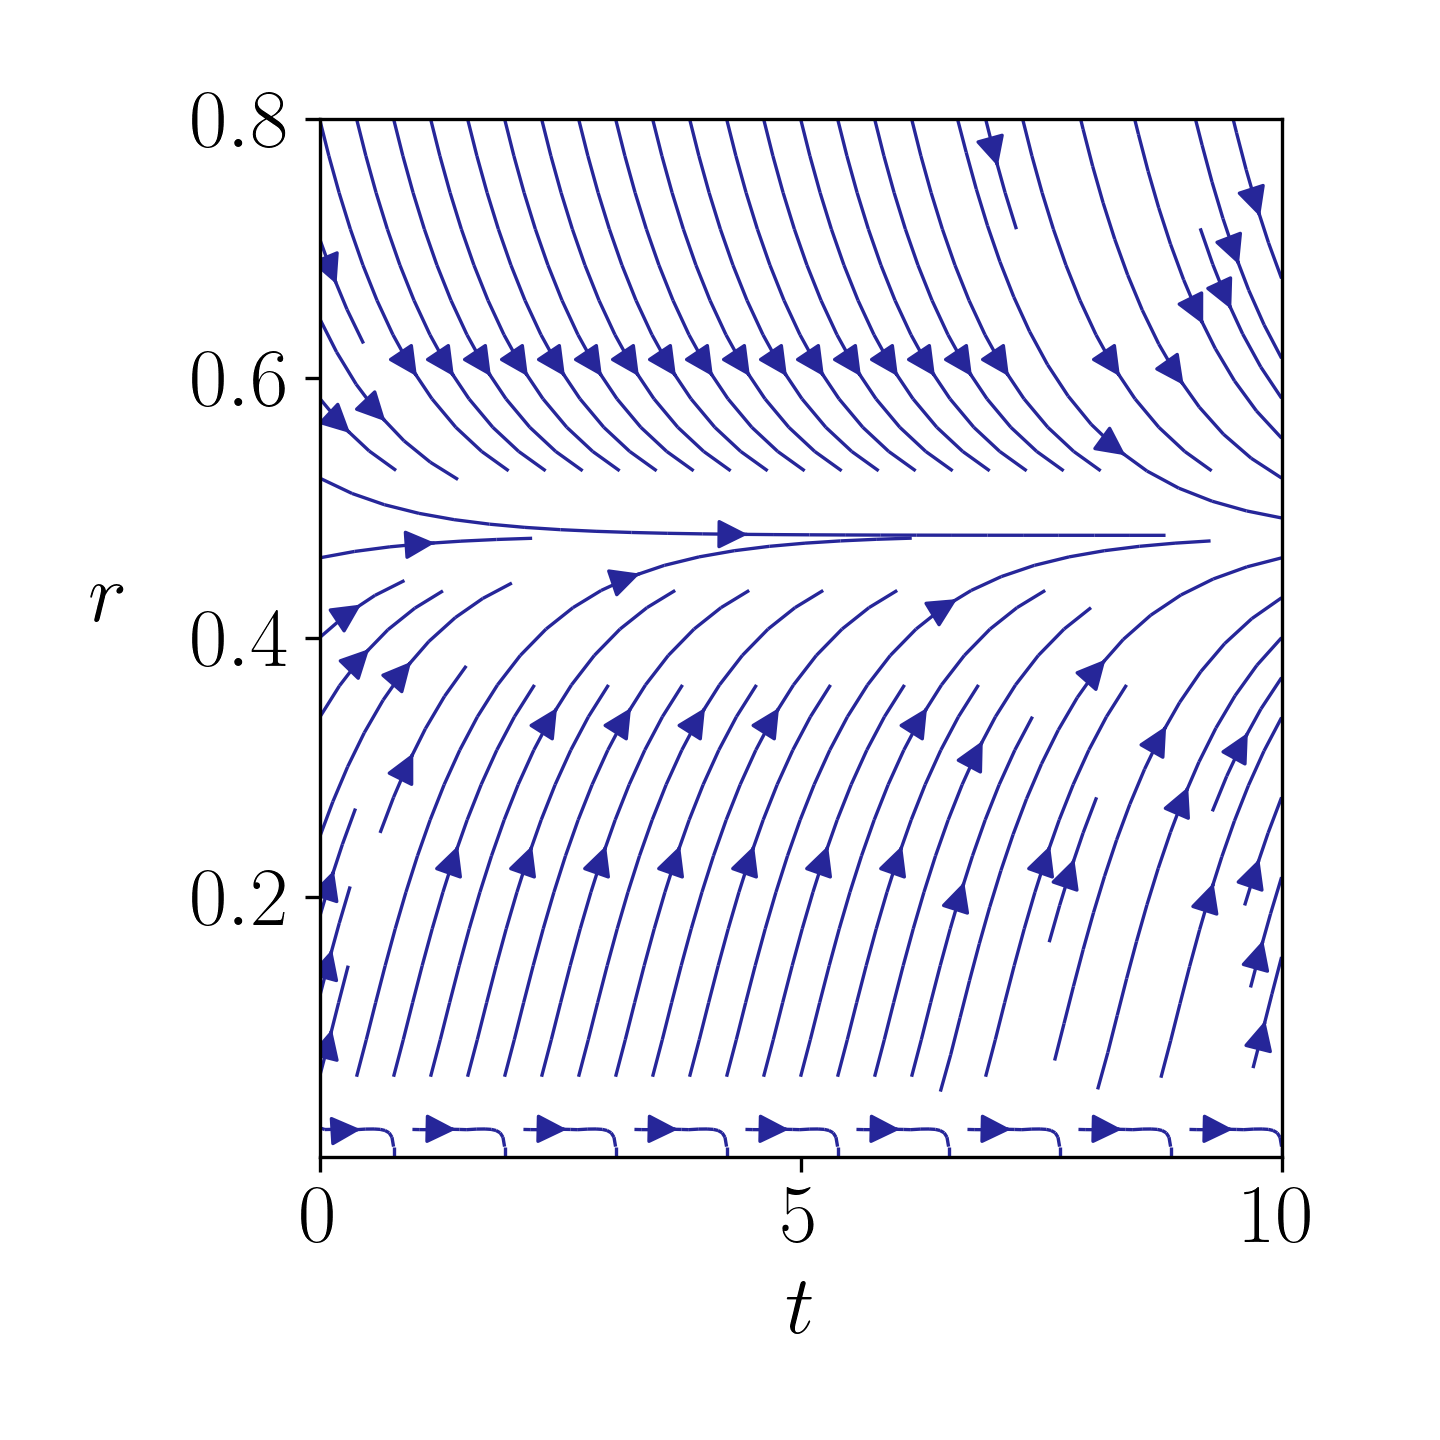
\includegraphics[width=\linewidth]{figures/streamlines/mod1-a99.png}
        \caption{$\alpha=0.99$} 
        \label{fig:radius-characteristics-99} 
    \end{subfigure} 
    \caption[Streamlines in the radially symmetric situation]{Streamlines for the zero level set curve, $\Gamma(t)$, in the radially symmetric situation with the pointset, \pointset, situated at $r_v=0.5$.}
    \label{fig:radius-characteristics}
\end{figure}

The motion of the streamlines can also be viewed in \figref{fig:radius-characteristics}, where we can follow the radius of the zero level set curves starting at a given radius, $r_0$.

We can also construct a general characteristic field for a situation with a fixed $\alpha$, point set radius $r_v$ and initial radius, $r_0$ by solving \eqref{eq:pde-streamline}. First we look at the term $\sigma(t) d(r)$ given the radius of the zero level set curve $r_{\Gamma}$
\begin{alignat}{3}
    \sigma(r_{\Gamma}, t)d(r) &= &|r-r_v| \qquad & \text{when }\radgammam \geq r_v \label{eq:sigma-radius-1}\\
    \sigma(r_{\Gamma}, t)d(r) &= -&|r-r_v| \qquad & \text{when }\radgammam < r_v \label{eq:sigma-radius-2}
\end{alignat}
Thus we can write \eqref{eq:pde-streamline} in terms of $r_\Gamma$ as
\begin{alignat}{3}
    r_t &= -&\bigg(\alpha |r(t)-r_v| + \frac{1-\alpha}{r(t)}\bigg) \qquad &\text{when }\radgammam \geq r_v \\
    r_t &= &\bigg(\alpha |r(t)-r_v| -  \frac{1-\alpha}{r(t)}\bigg) \qquad &\text{when }\radgammam < r_v,
\end{alignat}
Thus, the only thing we need in order to make the full characteristic field is to find the time when $r_{\Gamma} = r_v$, which can be found from \eqref{eq:streamline-solution} and \eqref{eq:streamline-solution-constant}.

This is done in \figref{fig:total-streamline-picture} for a curve starting with $r_0=0.6$ with a point set, $\mathcal{V}$, situated in $r_v=0.5$ and the weighting $\alpha = 0.96$. A useful formula when $(4-\alpha(r_v^2+4))<0$, which is also true for this case, is that the arctangent of an imaginary number is
\begin{equation*}
    \tan^{-1}(i x ) = \frac{i}{2} \ln\bigg(\frac{1+x}{1-x} \bigg).
\end{equation*}

In the figure, we see that the streamlines stemming from the area around the initial curve moves similarily to the zero iso-contours in \figref{fig:radius-characteristics-96}, but further away, they differ more and more. That is because the sign change of $\sigma(r, t)$ happens more and more out of sync with when that particular level set falls into the point set. 

We also observe in the \figref{fig:total-streamline-picture} that level curves in a band around the zero level curve approaches the stationary radius as well. When numerous level curves approach the same radius, the higher dimensional function becomes steeper and steeper. This can cause problems for a numerical scheme which is sensitive to steep gradients.


\begin{figure}
    \begin{subfigure}{.5\linewidth}
        \centering
        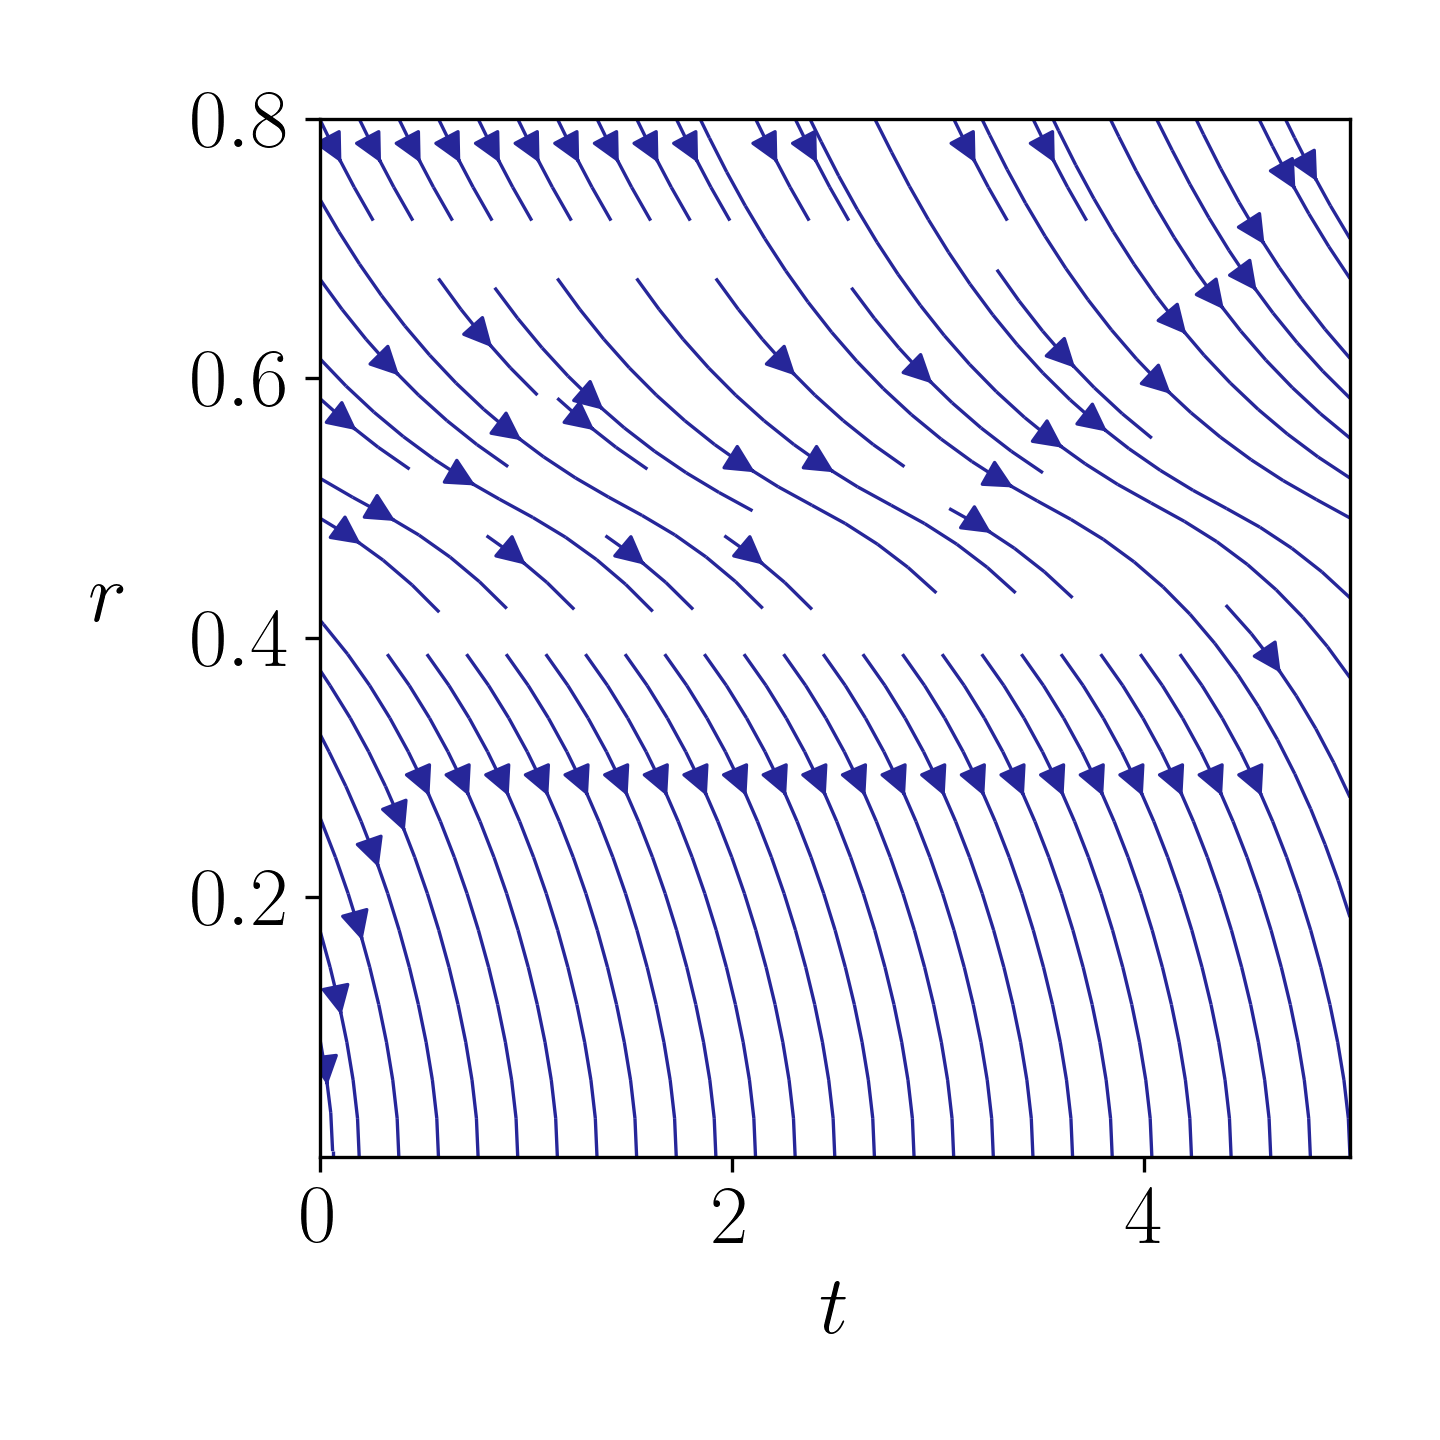
\includegraphics[width=\linewidth]{figures/streamlines/mod1-a96-pos.png}
        \caption{Streamlines with $\sigma(r, t) = 1$}
        \label{fig:sub1}
        \end{subfigure}%
    \begin{subfigure}{.5\linewidth}
        \centering
        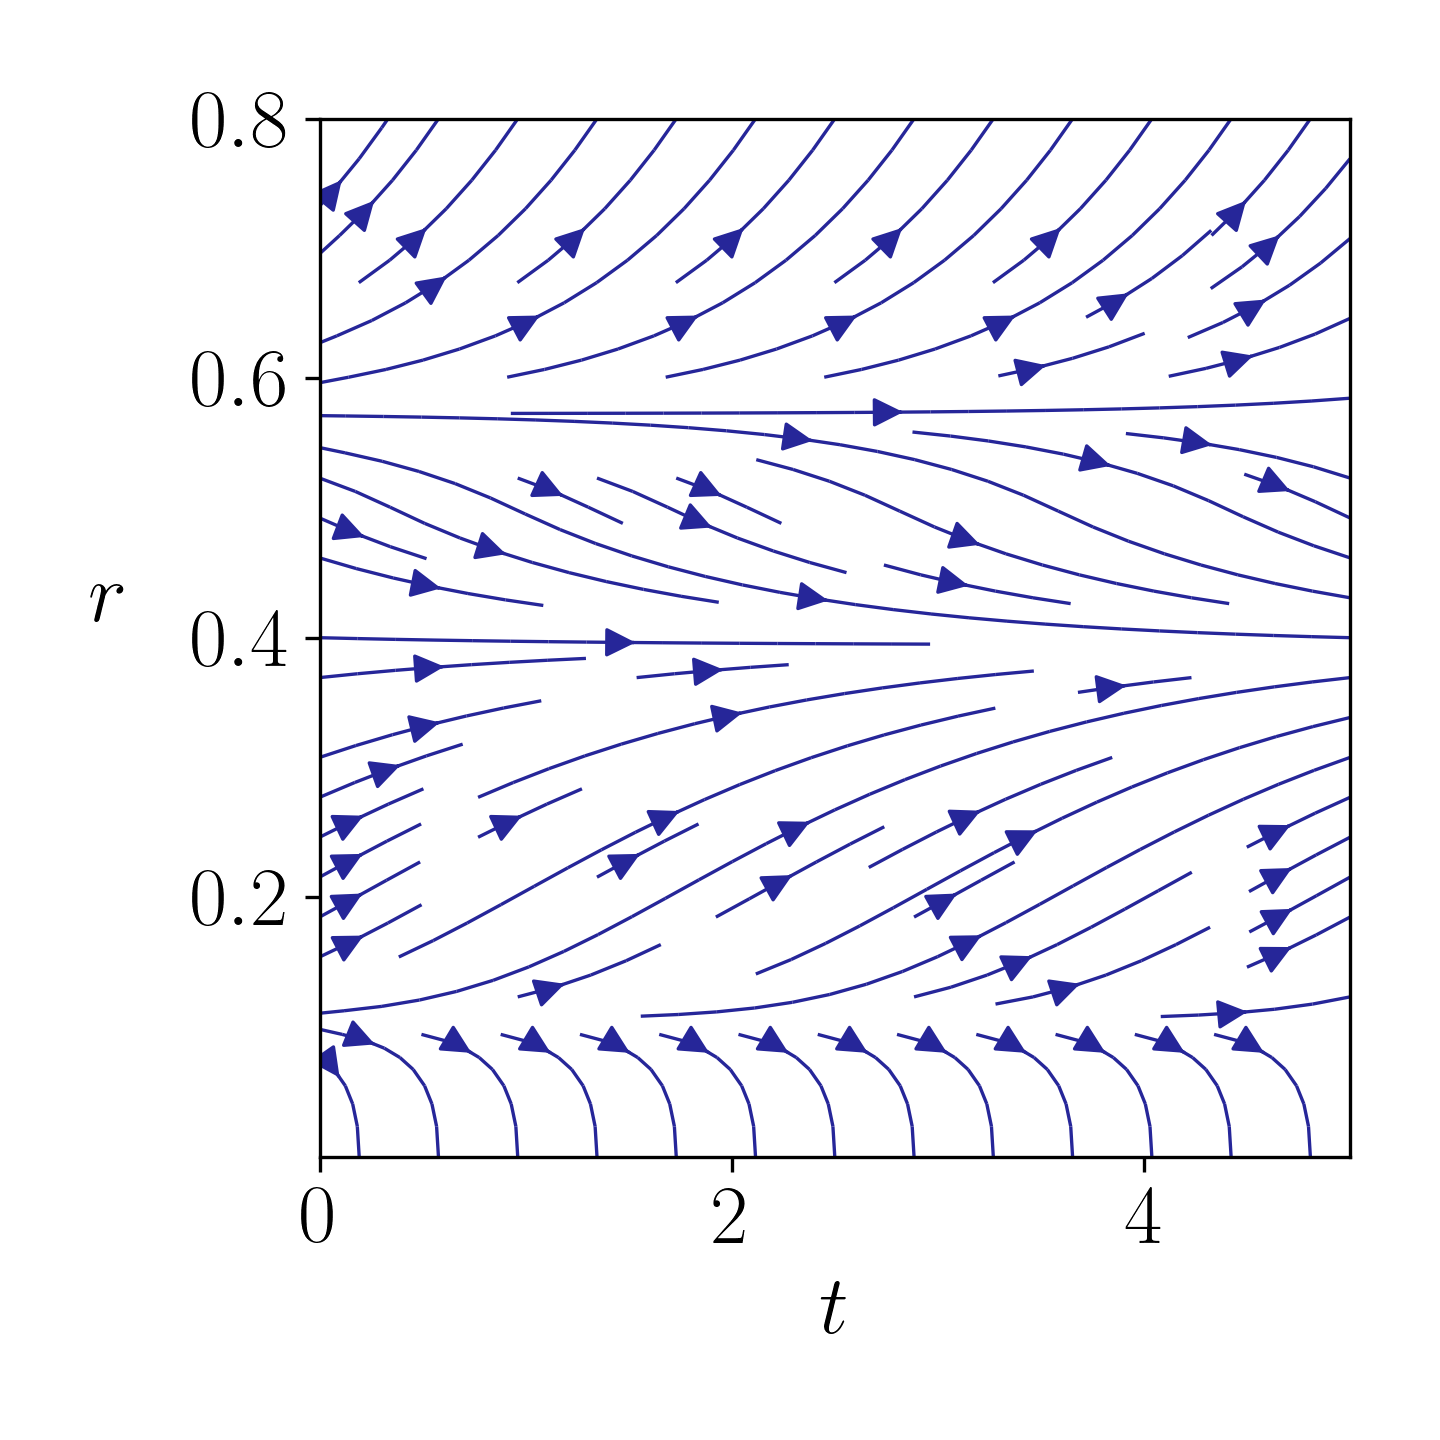
\includegraphics[width=\linewidth]{figures/streamlines/mod1-a96-neg.png}
        \caption{Streamlines when $\sigma(r, t)=-1$}
        \label{fig:sub2}
        \end{subfigure}\\[1ex]
    \begin{subfigure}{\linewidth}
        \centering
        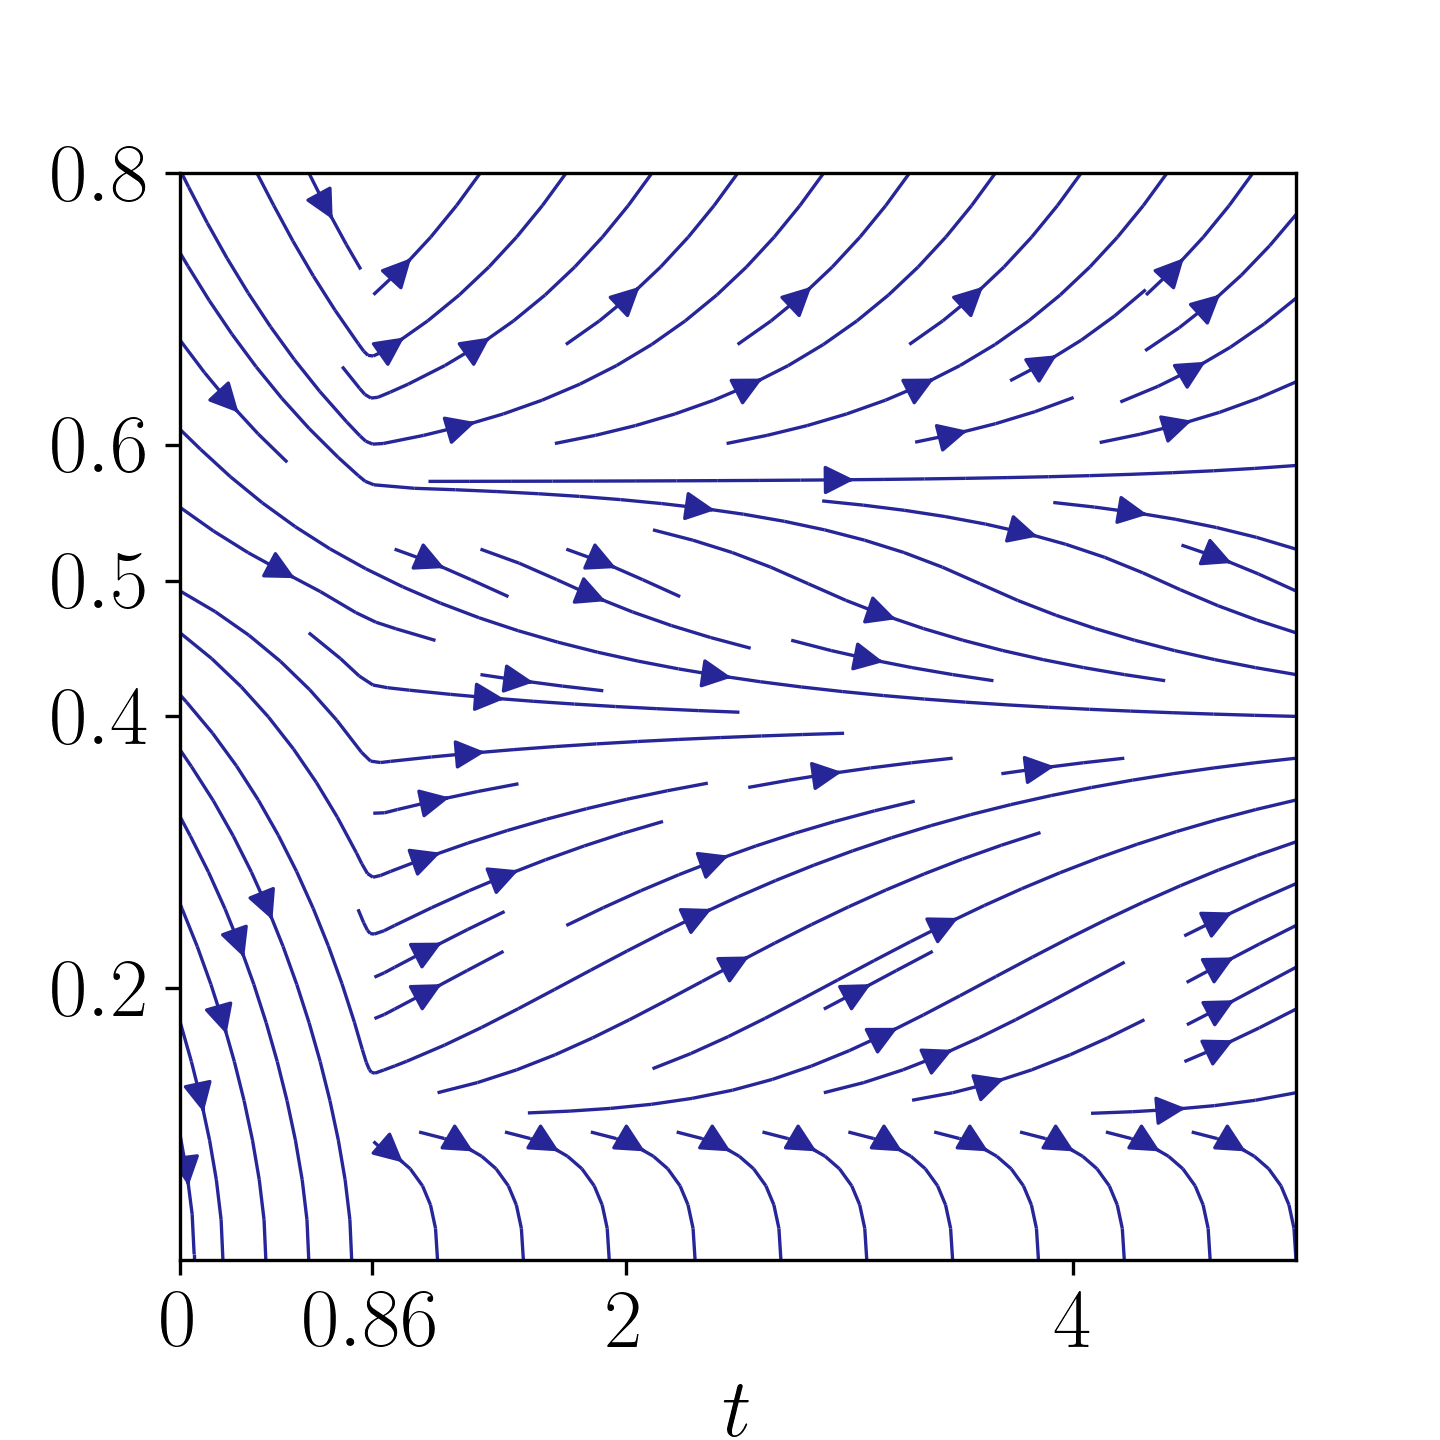
\includegraphics[width=.5\linewidth]{figures/streamlines/mod1-a96-tot.png}
        \caption{Streamlines for all level curves when the zero level set curve, $\Gamma (t)$ has initial radius, $r_0=0.6$.}
        \label{fig:sub3}
    \end{subfigure}
    \caption[Streamlines for all level curves]{Streamlines when the sign function is $\sigma(r, t) = +1$ and $\sigma(r, t) = -1$, for a point set with radius, $r_v=0.5$ and weight $\alpha=0.96$ on top. The lowermost figure shows the streamlines when the zero level set curve has initial radius $r_0=0.6$. Meaning that the sign of $\sigma(r, t)$ changes in $t=0.86$.}
    \label{fig:total-streamline-picture}
\end{figure}


